\subsection{Initial Simulations}\label{Section:Initial-Simulations}

First, we summarize the technical details:
\begin{itemize}
    \item A player is represented by their individual pool, which is a $152$-length bit array.
    A $1$ is present if the player owns the element and it is $0$ otherwise.
    \item Our simulator performs the scheme given in \Cref{Sec:Problem-Definition}.
    \item We run the simulator $100000$ iterations per instance of randomly generated pools (where one instance is $10$ players).
    Due to limited computational resources, we found that the gain in accuracy in performing more iterations was not worth the increase in time.
    To obtain the individual probability distributions, we keep track of the elements chosen per player and divide by $100000$ (the total number of iterations).
\end{itemize}

We randomly generated $300$ instances of our problem and ran them through our simulator with both a random ordering of players and a greedy ordering.
Then, we measured the Hellinger distance of the resulting distributions to the uniform distribution.
The aggregate results can be seen in \Cref{Figure:simulation-results-histogram}.

\begin{figure}[htbp]
    \centering
    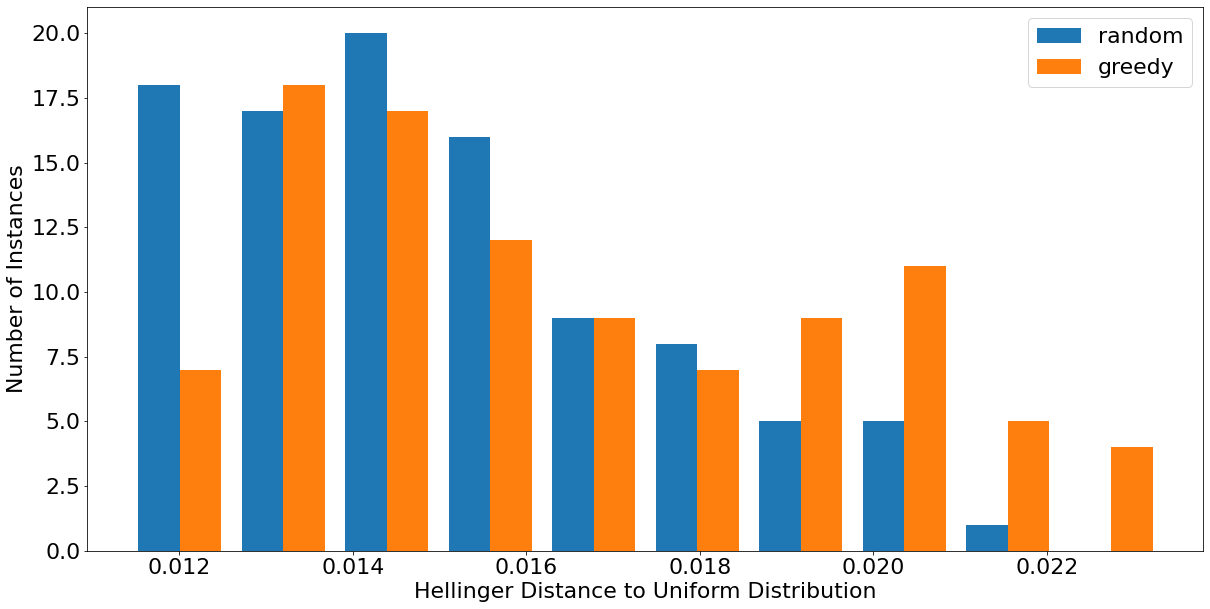
\includegraphics[width=.9\textwidth]{figures/simulations.png}
    \caption{Hellinger distance of simulated distributions to the uniform distribution using a random ordering and greedy ordering.}
    \label{Figure:simulation-results-histogram}
\end{figure}

Interestingly, the results show that the greedy ordering yields distributions that are \it{ever so slightly} less uniform than when using a random order.
This appears to contradict the conjecture we set out to gain evidence for!
However, as we noted previously, we only obtained $300$ samples out of the exponentially many possible instances of our problem.
There's nothing special about this number, we just decided to stop the simulations at a round number after several hours of computation.
The simulator scaled poorly with the number of iterations it was performing per instance.
For this reason, we were motivated to find some way to speed up the process of simulating our game.
This leads to the work done in the next section, where we completely replace the simulator with a neural network.